\chapter{Investigation of Visualization Tools using a Feature Classification Scheme}
\label{chap:Tools}

\section{Selection of Tools}\label{tool:selection}
In this section we analyze selected visualization tools in business and their ability to visualize large time-oriented data. Therefore, we developed a classification scheme which is based on the collected success criteria of chapter 3. \\*
As discussed in chapter 3 visualization tools need to provide scalable visualization techniques or the ability to extend the tool with custom visualizations. Moreover, Interaction and distortion techniques are necessary to improve scalability. Analytical methods reduce the amount of data vertically and horizontally. 
Advanced Data Visualization in business context requires software that is able to scale visualization in an "effective manner"\cite{Russom2011}. Offering advanced visualization techniques, parameterization, interaction and analytical methods such as data abstraction\cite{Tegarden1999,Aigner2011,Eick2002,Zhanga} are core functions of ADV software. \\*
\textbf{The Role of APIs}
Commercial software tends to need more time for the development and integration of advanced visualization for large data\cite{Zhanga, Simon2014}. To bridge the gap, vendors started to offer a bunch of APIs to create and integrate visualizations. 
% data load for BigData: 
\textbf{Software not included in this work}
As the goal of this work is to compare visualization tools in business we only consider software which is 
\begin{enumerate}
    \item generic: not specialized to one domain
    \item integrates visualization features
\end{enumerate}

Furthermore, the software needs visualization features, the ability to present time-dependent data. Software with one of the following items is intentionally not considered: 
\begin{enumerate}
    \item Software that only presents one-dimensional data. 
    \item Software that is specialized to data mining.
\end{enumerate}

Based on the Magic Quadrant for Business Intelligence and Analytics Platforms 2017 \cite{Sallam2017} Qlik, Tableau and Microsoft are the leading visionaries of BI Vendors. \cite{ITCentralStation} as a crowdsourcing recommendation platform for BI tools ranked Tableau, Qlik, Oracle, Microsoft Power BI and IBM Cognos on the first five places. Nevertheless, marketrelevance reports from Gartner, Forrester, Barc and other so called "research and advisory companies" usually do not publish a detailed scoring model. Thus, the ranking might not be appropriate to our needs.

Eventhough, Qlik, Tableau and Power BI are ranked as BI tools they can call themselves visualization tools. 
Thus, we chose the tools: Power BI, Tableau and Qlik Sense (QS).\\*
Moreover, we added d3.js as this javascript library is open-source, state-of-the art in visualization and offers a wide range of visualization possibilities.

Even though the selection of the tools is not exhaustive, we believe that the reviewed products represent the state-of-the art and provide the table of different tools which was used for chosing the remaining 5 tools in the appendix.

\subsection*{Qlik Sense}
Qliktech was founded in 1993 with the goal to "mimic how the brain works."\cite{qlikHistory}. They offer five products(QS, QS Cloud, QlikView, QlikView NPrinting, Qlik DataMarket) and the Qlik Analytics platform. QS 1.0 was released in September 2014 for visual analytics. 
\todo{evlt. raus}
It offers functions such as Smart Data Load which allows to load large data from different data sources.

\subsection*{Power BI}
Microsoft Power BI came alive in ...\todo{datum einfügen}. It is made up of six main components: 
\begin{enumerate}
    \item Power Query: Data Mesh-up tool
    \item Power Pivot: Data Modelling Tool
    \item Power View: Data Visualization Tool
    \item Power Map: 3D Geo-spatial data visualization tool
    \item Power BI Desktop: Reporting Tool 
\end{enumerate}
These components can be combined for interactive data analysis. In our work we will focus on the data visualization tool: Power View. We will briefly discuss Power Pivot in the context of database metrics. 

\subsection*{d3.js}
d3.js is a javascript library used for visualization. It visualizes data based on SVG, HTML5 and CSS and binds data to existing web elements in alignment with the Document Object Model (DOM).  Data Handling is managed by the underlying data source, data modeling can be handled by other javascript libraries such as node.js. A good overview how d3.js works is given in \cite{Meeks}. 
We chose d3.js as it is a data visualization tool with interaction. As it is free it becomes an alternative to commercial tools.

\subsection*{R}
R is a free and opensource language for statistical computing and graphics. Its modular structure consisting of many packages makes R highly extendable\cite{R}. Some packages enable the user to do analytics with R, others support different visualization techniques. Usually those packages also support interaction except the user additionally uses other libraries such as plot\_ly() or Shiny. Both of them are frameworks which combine R graphics with interaction techniques. Besides of that some packages offer interaction techniques, e.g. dygraphs(), while others do not. Thus, our classification scheme is only valid combined with specific packages.
There exists many packages which treat time-series data, e.g. \textit{zoo} and \textit{dygraphs} treat time-series. Large data sets are handled in \textit{bigvis}.

\section{Scalability of visualization tools}\label{tool:scalability}
The scalability of visualization tools is measured by the \text{visualization characteristics} and the \textit{database metrics}. Moreover, as discussed in \ref{chap:BIV} important features are interaction techniques and analytical methods. 

\subsection{Database metrics}
According to Eick visual scalability is not only determined by the visualization characteristics but also by the database metrics. Eick defined database metrics as the size of the database which can be handled by tools\cite{Eick2002}. One possibility to measure the database size are the number of lines which can be load into the tool and the limitations on visualizations in the number of rows.\\*\\*
While \textbf{Tableau} and \textbf{Power BI} have no limitations how many data can be loaded, \textbf{QS} inherits the data load limitations of Qlik View: A QS document cannot have more than 2,147,483,648 distinct values in one field. This limitation still allows Qlik to handle large and huge data sets according to our definition. Moreover, 2 billion data points exceed the limit of screen pixels. But nevertheless, QS is outperformed by Tableau and Power BI in this particular case.
\\*\\*
In context of visualization the number of rows which are loaded into a visualization is a determining factor for scalability. For large data the user expects to load all data he wants the tool to load. However, some tools limit the initial number of rows and the user has to write additional code. This effects the easy-of-use negatively.
QS limits the initial fetch to 10.000 but gives the opportunity to fetch more data if needed. \textbf{Power BI} and \textbf{Tableau} currently have no limit for rows in visualization.
Again QS stays behind Tableau and Power BI.
d3.js 

\subsection*{More than database metrics}
Nowadays, data management shifted from importing csv-files or Excel Spreadsheets to storing data sets in technologies such as clouds or databases. 
Therefore, most of the visualization tools provide data engines, an underlying software component which manages the data. Thus, the tool performance depends at the following factors:
\begin{enumerate}
    \item Hardware Resources
    \item the underlying engine
    \item perceived performance 
\end{enumerate}
In our understanding of visual scalability Eicks definition of database metrics needs to be adjusted in a way that it meets the characteristics of tools today. Thus, we expand \textbf{database metrics} by the ability to integrate data storage.

\textbf{In-memory versus Real Time Connection}
In-memory techniques store their data inside the RAM while real time technologies work directly on the database.
With large data sets in-memory technologies might not be feasible. Eventhough, working in-memory is faster than working directly at the database. With a smaller subset of large databases working in-memory might be the better option. 
\textbf{QS} data engine (QIX Engine) and \textbf{Power BI} use in-memory columnbased technology. While the data engine processes calculation the RAM may be temporarily allocated. Thus, QS is limited by the primary memory of the computer. \textbf{Power BI} also connects live to clouds and on premises similar to \textbf{Tableaus} Data Engine which is designed to work live on the database. At Tableau data extracts can be created to work in-memory. The limits for data extracts are not published but Tableau Public, the free version of Tableau, recently extended the limit of 1 mio. rows to 10 mio. rows in-memory. 
For working with large data sets Tableau again outperformed QS and Power BI.\\*
\textbf{Connection to multiple data sources}
With large data sets data is distributed about several places. The ability to connect to multiple databases impacts the scalability. All of the tools can connect to multiple data sources. In future work, a performance review for the connection of the tools to multiple data sources is recommended.\\*
\textbf{Incremental Loading}
With large data sets tools might be overstrained with loading the whole data sets at once. Strategies to tackle this problem are incremental load. \textbf{QS} uses a custom data model called .QVD files. In .QVD files data is highly compressed and allows incremental loading. Tableau allows the incremental refresh of data extracts which adds only new rows to the extract. Power BI does not offer the option of incremental loading. 
\textbf{Further Aspects}
Scalability of tools can also be measured in terms of users and delivery which goes beyond our scope.




\subsection{Visualization Characteristics}
In the context of \textit{visualization characteristics} QS, Tableau, Power BI and d3.js have been compared regarding \textit{Visualization Techniques, Analytical Techniques and Interaction Techniques}. 

\subsection*{Qlik Sense}

\subsubsection*{Visualization Techniques}
QS offers 8 built-in visualization techniques: bar charts, line charts, pie charts, scatterplots, treemap, maps, combi charts and gauge charts. If an additional technique is wanted the user can either use one of the community's self-made extensions or he can build his own visualization extension with \textit{javascript} and \textit{QEXT} files\cite{qlikWorkbench}. QS provides an extension template which supports the user in writing its extensions. Moreover, Qlik provides 20 high-level-APIs which supports the user in writing a custom extension. However, the user needs to know javascript and html\cite{qlikVisExtensions}, as well as QS own QEXT-language. \\*
Out of the QS standard repertoire non of the visualization technique corresponds to the studied visualization techniques of chapter \ref{chap:BIV}. With d3.js it would be possible to build these visualization techniques and integrate them in QS. 
The embedding of javascript also allows \textbf{Aggregation} in terms of multi-resolution and the use of aggregation markers. However, this again requires coding-skills. 

In the field of built-in-aggregation markers QS offers data aggregation for one chart type: the scatterplot. Hereby, large data is aggregated by aggregation markers. When the scatterplot is shown at an overview level accumulated data points are represented by squares. The color shows the data items density. The darker the square the denser the data\cite{qlikScatter}. With the so called \textit{Smart Data compression} Qlik starts to consider large data amounts. However, offering Smart Data Compression only for one technique Qlik stays behind the present day requirements.


\begin{figure}[H]
    \centering
    \subfloat[QS]{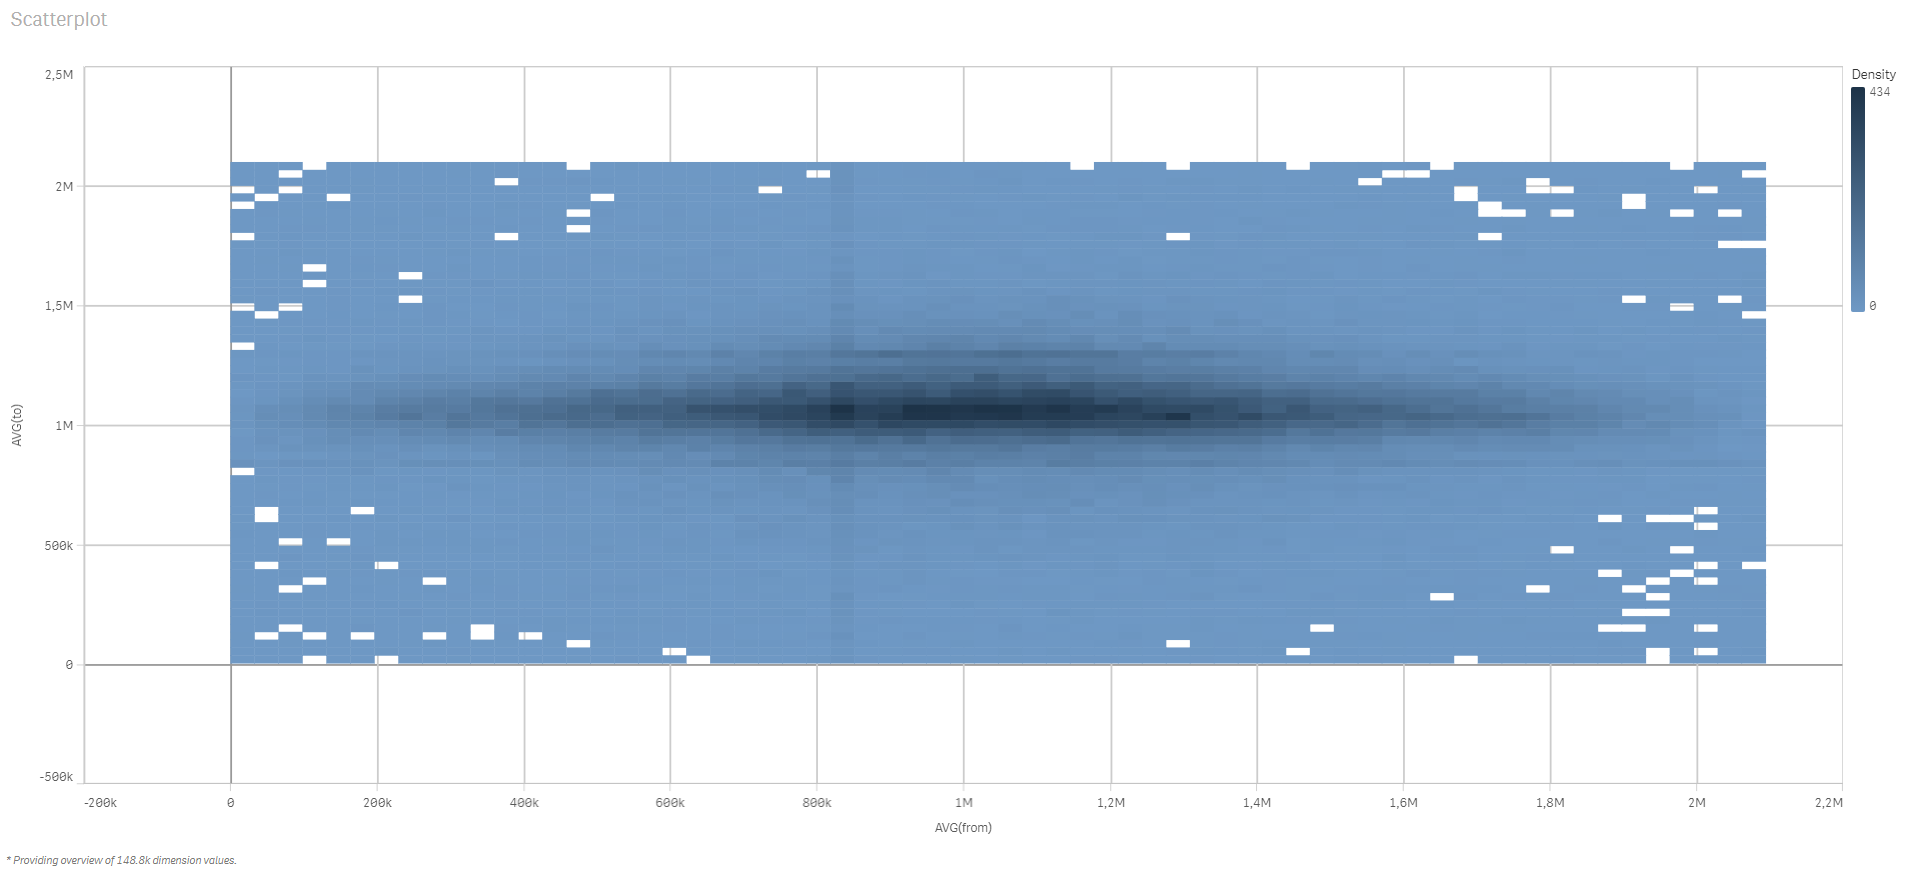
\includegraphics[width=6cm]{src/images/SmartDataCompression}}
    \caption{Smart Data Compression (left): Overview level which shows aggregated data points by squares and color and changes the shape if zoomed in}
    \label{fig:smartdatacompression}
\end{figure}

\begin{figure}[H]
    \centering
    \subfloat[Sparse Area]{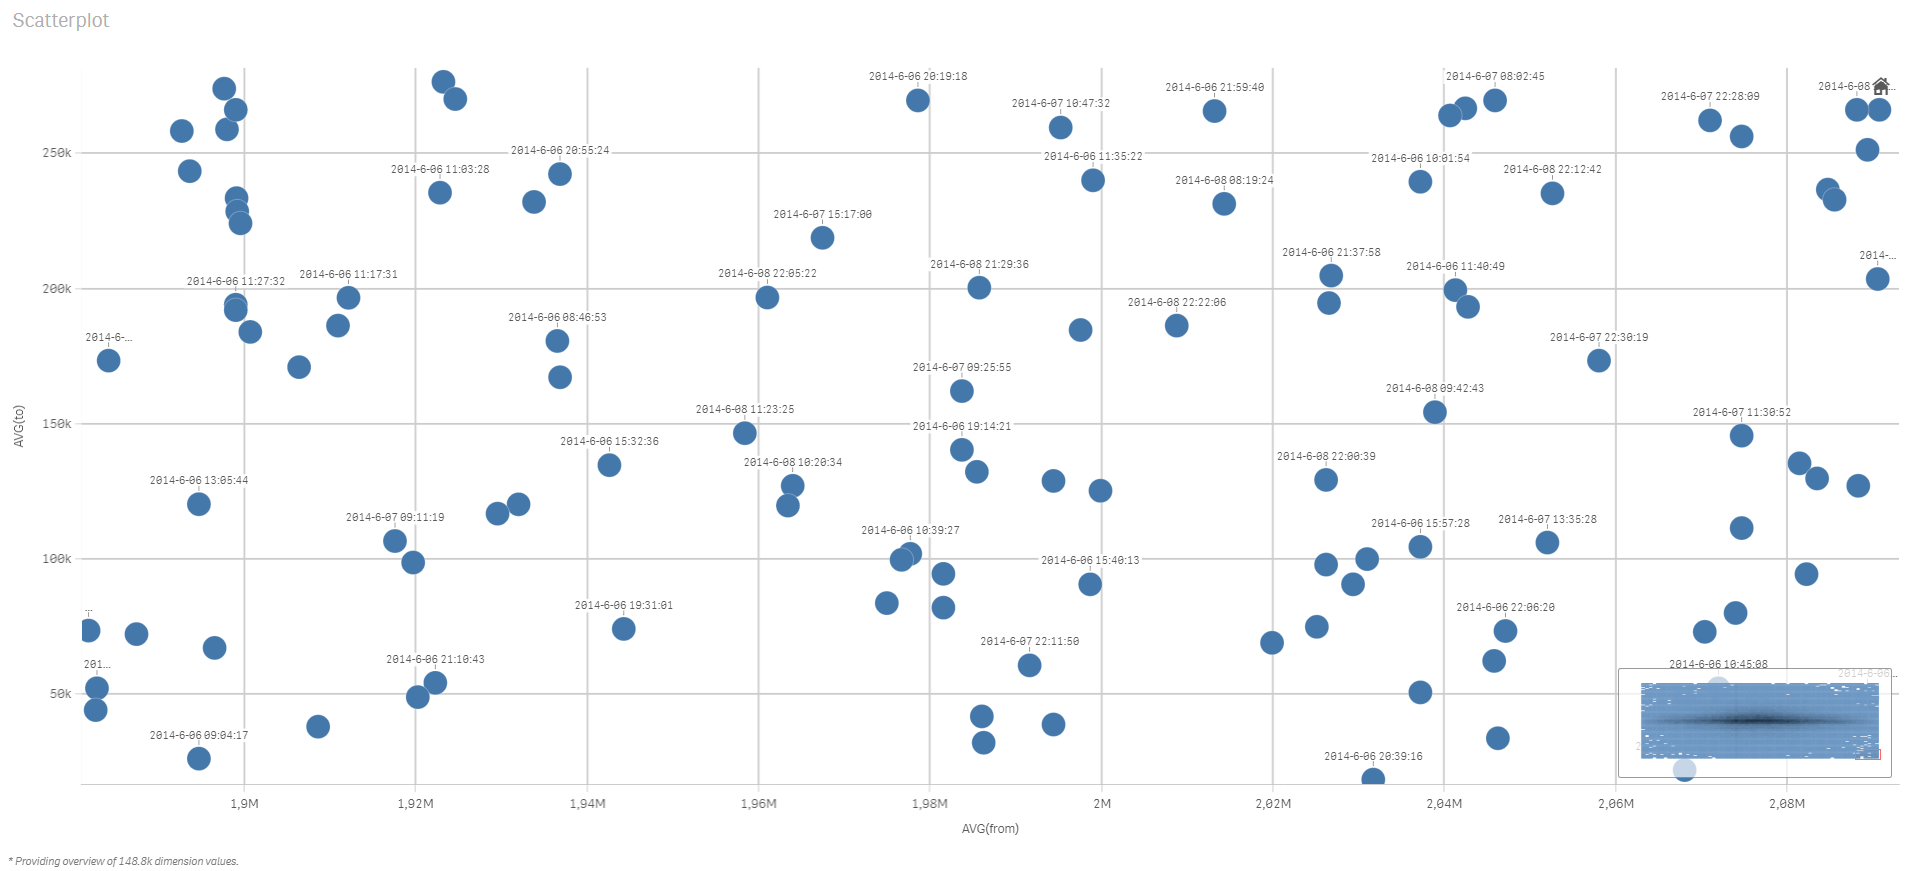
\includegraphics[width=6cm]{src/images/SmartDataCompressionI}}
    \qquad
    \subfloat[Dense Area]{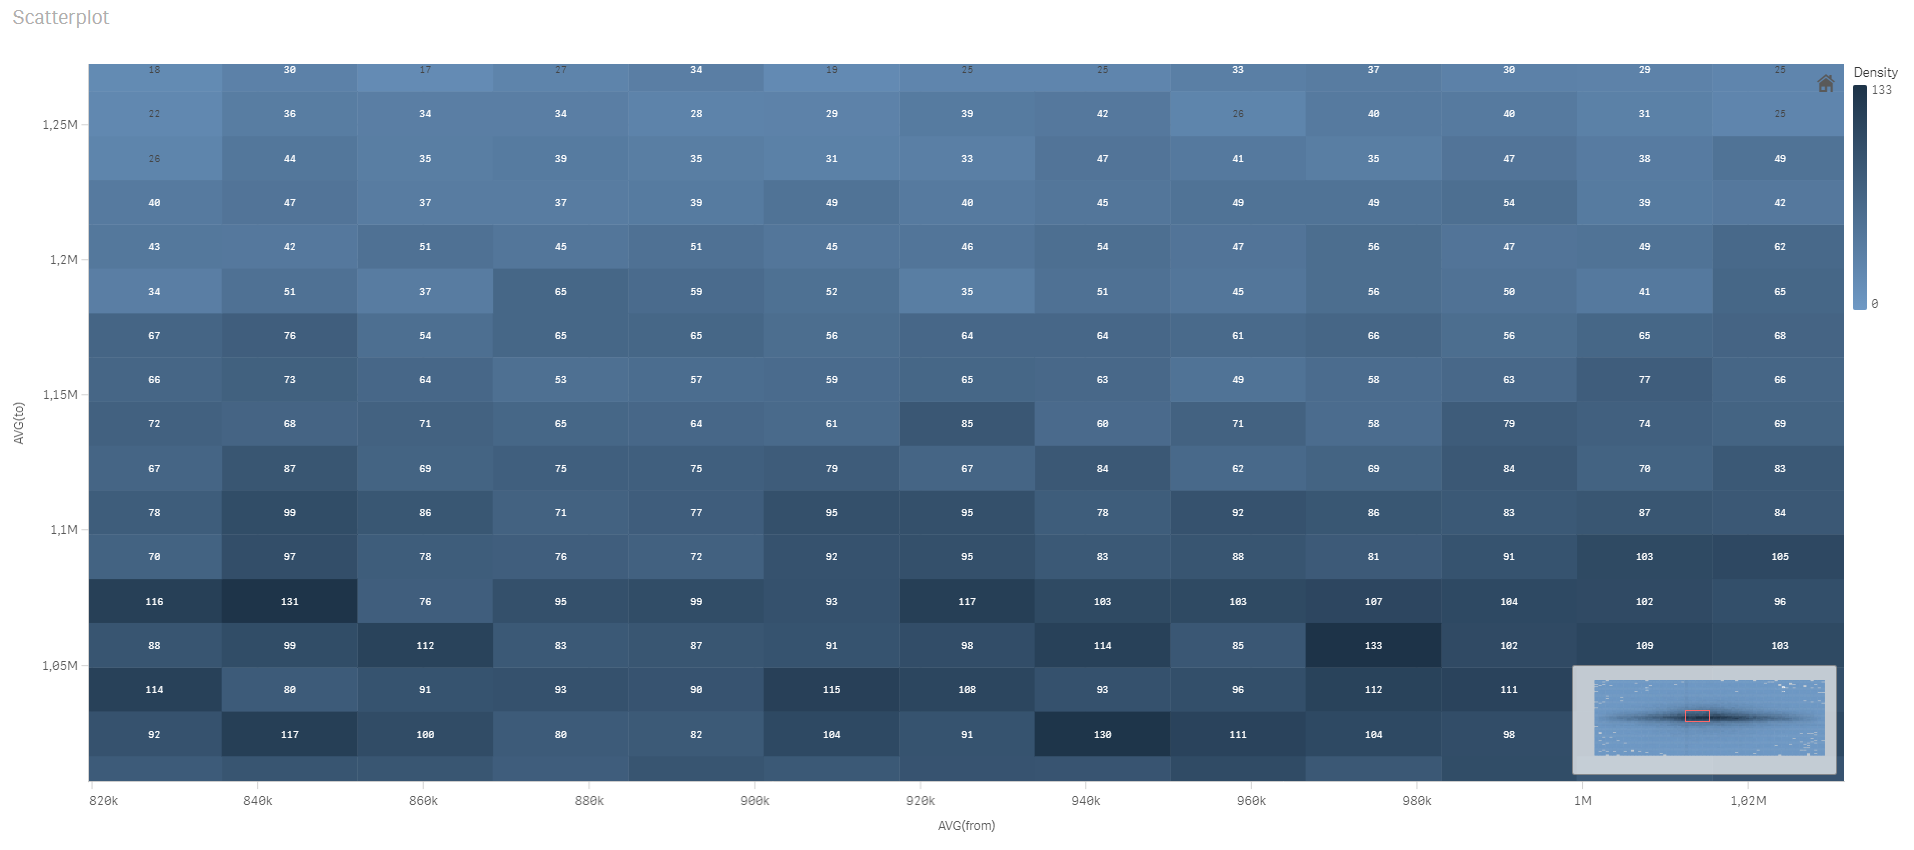
\includegraphics[width=6cm]{src/images/SmartDataCompressionII}}
    \caption{Smart Data Compression: Detail level}
    \label{fig:smartdatacompression}
\end{figure}

\subsubsection*{Analytics}
Data reduction is part of QS Server. With dynamic data reduction rows can be hidden for a group of users. Thus, data size is decreased. Internally, .QVD files compress data. But, the user cannot reduce data size based on an interactive selection inside the dashboard. In this case, the user could select a group of data and decide whether he wants to keep only the selected data. 
QS implements \textbf{Aggregation} with aggregation-functions. These use QS specific set expressions and range from basic statistical functions (min,avg,max) over financial functions, to advanced statistical functions(linear regression, correlation). With these aggregation functions QS offers some analytical methods. Yet, QS has no integration to an analytical program.
\subsubsection*{Interaction}
To allow a focus + context view QS offers navigational maps\cite{beard1990navigational} which come as navigational slider in which a miniature version of the whole data set\cite{beard1990navigational} is shown. 
Filters can be applied by making selections or dragging a filter inside the visualization\cite{qlikSheet}  and all views then are adapted to the current selection. Thus, QS offers Brushing + Linking. An additional linking-feature are \textit{master items}\cite{qlikChangeData}, which allow the user to change properties for all master items at once.
For details the user can search QS with Smart Search in which the dimensions, measures and metadata is searched and visualizations ,tables and KPIs are displayed\cite{qlikSmart}.  


\subsection*{Tableau}
The Tableau approach to large data visualization is \textit{extract data first, then visualize}. This approach is manifested in the fact, that some functionalities in Tableau are only available for data extracts. Count distinct, offline access and incremental refresh are these features.
Tableau published a guideline "Best Practises for Designing Efficient Tableau Workbooks" in which they recommend of showing the highest aggregation level first and show only a selection of records. This approach basically implements Shneidermans \textit{Overview first, zoom-in and filter, then details on demand.} and influences also the strategy for large data visualization: a focus in analytical methods. 

\subsubsection*{Visualization Techniques}
Tableau offers 22 built-in visualization techniques: heat maps, symbol maps, stacked bars, pie charts, horizontal bars, side-by-side bars,treemaps,circle views, side-by-side circles, continuous lines, discrete lines, dual lines, area charts,  discrete area charts, dual combination, scatter plots, histogram, box-and-whisker plots, Gantt chart, bullet graphs and packed bubbles.
Visualization extensions are not possible even though Tableau has a Javascript API. This API allows the integration of a Tableau dashboard into a web page, but is not built for writing javascript extensions for Tableau. Besides the number of technique, advanced metahpors such as multi-resolution, data abstraction or aggregation markers are not supported. 
In sum, Tableau is a well-known choice in the visualization community. But it does not support large scale visualization features. 

\subsubsection*{Analytics}
Tableaus analytical strategy is manifested in the support of analytical functions. On the one hand, Tableau offers build-in modelling functions: prediction, trend line, cluster, average and median. Furthermore, R scripts can be loaded into Tableau.  
In terms of data reduction data extracts can be loaded in Tableau and filter can be applied. Sampling also can be achieved by using aggregation functions. Sampling based on the selection is not possible.

\subsubsection*{Interaction}
Regarding interaction Tableau offers Brushing&Linking, Zooming and Filtering. Furthermore, Tableau supports Pan & Zoom. 
Distortion techniques such as graphical fish-eye or bifocal displays are not supported. 

\subsection*{Power BI}

\subsubsection*{Visualization Techniques}
Microsoft Power BI offers 8 built-in visualization techniques, 15 available techniques at the MarketPlace and 75 visualization apps in the visuals gallery. Additionally, the user can build custom visualization apps by writing \textit{TypeScript} or \textit{R}. Out of the 98 techniques none of them implements any discussed techniques of chapter \ref{visualization}. Moreover, so far advanced Metaphors are not supported\cite{Amanda}. One approach to aggregation markers are \hyperlink{https://Power BI.microsoft.com/de-de/blog/power-bi-desktop-october-feature-summary/#grouping}{\textit{Groups}} which can be combined with drill-down options.

\subsubsection*{Analytics}
Data Reduction in Power BI is possible with a data view on the database which considers less data than before. Moreover, data sets can be extracted with the \hyperlink{https://Power BI.microsoft.com/de-de/blog/power-bi-desktop-october-feature-summary/#grouping}{\textit{Inclusion/Exclusion}} of data points.\\*
\textbf{Integration of analytical program:} Besides the own core functions for data reduction Power BI is connected to analytical programs such as \hyperlink{https://Power BI.microsoft.com/de-de/blog/power-bi-desktop-october-feature-summary/#grouping}{\textit{R, Mixpanel or comScore.}}\\*
\textbf{Aggregation and Sampling} for example can be achieved in embedding R scripts or in using calculated fields. \\*
\subsubsection*{Interaction}
With cross-highlighting Power BI includes brushing and linking\cite{Power BIInteract}. Moreover, filter functions are embedded. The \textit{focus mode} expands one visualization to full screen and thus, enables the user to have a detailed view on the visualization. The app \textit{Advanced Time Slicer} is one implementation of the distortion technique navigational map for time-oriented data. Navigation in Power BI is also realized by the search mechanism Power Q&A which answers NLP-question regarding the data set. Power Q&A includes filtering with the keywords WHERE, AFTER, BEFORE, BETWEEN, WITH or by naming the date as well. 

\subsection*{d3.js}
\subsubsection*{Visualization Techniques}
In d3.js data attributes are assigned to graphical attributes. It has not only one way to present pie charts but offers functions which process the data set in a way that pie charts can be drawn. This comparison is valid for other techniques but pie charts. By writing javascript code any visualization technique any advanced metaphor can be implemented. Some examples are d3.hexbin which allows binning,  simplify.js for data abstraction or clusterfck for clustering.  
Marker clustering in d3.js can for example be achieved with \href{https://www.phase2technology.com/blog/using-d3-quadtrees-to-power-an-interactive-map-for-bonnier-corporation/}{quadtrees}\cite{Morrison2014}. Simplify.js for example reduces data points on polylines while maintaining the characteristic shape of the polyline. This is one example for data abstraction.

\subsubsection*{Analytics}
While d3.js is only designed to visualize data it does not inherently offer the ability to analyze data. Therefore, a number of javascript libraries exist which can be combined with d3.js. Some examples are simplestatistics.js, regression.js, node.js with the packages data-reduction, ml-pca or dimensionality-reduction. 
As javascript allows the integration of libraries there is basically no limit for analytical functions. 

\subsubsection*{Interaction}
d3.js allows to integrate various interaction techniques such as Zooming, Filtering or Linking \& Brushing. Distortion techniques can be achieved with the d3 plugin \hyperlink{https://bost.ocks.org/mike/fisheye/}{\textit{Fisheye Distortion}}\cite{Bostock2012} which allows circular, linear and logarithmic distortion.
Perspective walls can be implemented with \hyperlink{https://bl.ocks.org/mbostock/10571478}{\textit{Perspective Transformation}}\cite{Bostock2017}.

\subsection{The classification scheme}\label{tool:classification}
The tools basis of assessment concerning \textit{visualization characteristics} is the classification scheme. The aspects \textit{Visualization Techniques, Analytical Techniques, Interaction Techniques} are assessed according to the criteria of completeness and required programming skills. The consideration of programming skills in business is important as the standard visualization tool user in a company may have few programming knowledge (compare \ref{user}). Moreover, investment costs in tools also increase the higher the required programming skills.

The criteria completeness and programming skills have been combined in the tool criteria score(TCS). Each tool has been assigned a tuple-sore: (Programming Skills, Completeness). If the assessed aspect did not exist 0 was assigned.

\begin{table}[th]
	\centering
	\caption[programming-skills]{Criteria Required Programming-Skills to use the assessed aspect}
	\label{programming-skills}
	\begin{tabu}{cl}
	\toprule
	Points & Criteria\\
	\midrule
	1 & Automatic support by tool \\
	2 & Available by drag and drop\\
	3 & Feature can be programmed in a popular programming language (R,Javascript,Java) \\
	4 & Feature can be programmed, but in a tool-specific programming language \\
	\bottomrule
	\end{tabu}
\end{table}

\begin{table}[th]
	\caption[completeness]{Criteria Completeness: extend to which assessed aspect is implemented in tool}
	\label{programming-skills}
	\begin{tabu}{cl}
	\toprule
	Points & Criteria\\
	\midrule
	0 & Not existing\\
	1 & 25\% completed \\
	2 & 50\% completed \\
	3 & 75\% completed \\
	4 & 100\% completed \\
	\bottomrule
	\end{tabu}
\end{table}

%example grid
\begin{figure}[H]
\centering
\scalebox{.75}{
    \begin{tikzpicture} 
        \begin{axis}[
        axis y line     = left,
        axis x line     = bottom,
        grid,
        grid style = {color=gray!50, dotted},
        xticklabels={,,1,2,3,4},
        yticklabels={,0,1,2,3,4},
        xmin       = 0, xmax = 4,
        ymin       = 0, ymax = 4,
        xlabel={Programming-Skills},ylabel={Completeness}
        ]

        \node at (axis cs: 1,2)   {Tool 1};
        \node at (axis cs: 3,3)   {Tool 2};
        \end{axis}
    \end{tikzpicture}}
    \caption{Tool Criteria Score (TCS)} \label{classification}
\end{figure}


\subsection*{Analytics}
%%% Horizontal Data Reduction
\begin{figure}[H]
\subfigure[Supports Analytical Functions]
{
    \begin{tikzpicture}[scale=0.55]
        \begin{axis}[
        axis y line     = left,
        axis x line     = bottom,
        grid,
        grid style = {color=gray!50, dotted},
        xticklabels={,,1,2,3,4},
        yticklabels={,0,1,2,3,4},
        xmin       = -0.1, xmax = 4.2,
        ymin       = -0.1, ymax = 4.2,
        xlabel={Programming-Skills},ylabel={Completeness}
        ]
        % (1) Supports Analytical Functions
         \addplot [] coordinates{};
        \node[rectangle with four colors, top color=red!50, right color=red!50, bottom color=red!50, left color=red!50,
        draw]  at (axis cs: 3,4) {}; %d3.js
        \node[rectangle with four colors, top color=green!50, right color=green!50, bottom color=green, left color=green,
        draw]  at (axis cs: 4,1) {}; %QS
        \node[rectangle with four colors, top color=yellow, right color=yellow, bottom color=yellow, left color=yellow,
        draw]  at (axis cs: 1,1) {}; %Power BI
        \node[rectangle with four colors, top color=blue!50, right color=blue!50, bottom color=blue!50, left color=blue!50,
        draw]  at (axis cs: 1,1) {}; %Tableau
        \node[rectangle with four colors, top color=blue!50, right color=blue!50, bottom color=blue!50, left color=blue!50,
        draw]  at (axis cs: 4,2.5) {}; %Tableau
        \end{axis}
    \end{tikzpicture}
}    
\subfigure[Integration of analytical program]
{  
    \begin{tikzpicture}[scale=0.55]
        \begin{axis}[
        axis y line     = left,
        axis x line     = bottom,
        grid,
        grid style = {color=gray!50, dotted},
        xticklabels={,,1,2,3,4},
        yticklabels={,0,1,2,3,4},
        xmin       = -0.1, xmax = 4.2,
        ymin       = -0.1, ymax = 4.2,
        xlabel={Programming-Skills},ylabel={Completeness}
        ]
        % (2) Integration with analytical program
        \addplot [] coordinates{};
        \node[rectangle with four colors, top color=red!50, right color=blue!50, bottom color=yellow, left color=white!50,
        draw]  at (axis cs: 3,4) {}; %d3.js, Tableau
        \node[rectangle with four colors, top color=green!50, right color=green!50, bottom color=green, left color=green,
        draw]  at (axis cs: 0,0) {}; %QS
        \end{axis}
        \begin{customlegend}[
            legend entries={ % <= in the following there are the entries
                d3.js,
                Power BI,
                QS,
                Tableau
            },
            legend style={at={(13.5, 5.5)},font=\footnotesize}] % <= to define position and font legend
            % the following are the "images" and numbers in the legend
            \addlegendimage{mark=*,red,opacity=0.5}
            \addlegendimage{mark=*,yellow,opacity=0.5}
            \addlegendimage{mark=*,green,opacity=0.5}
            \addlegendimage{mark=*,blue,opacity=0.5}
        \end{customlegend}
    \end{tikzpicture}
}
\caption{TCS regarding Horizontal Data Reduction} \label{TCShorizontal}
\end{figure}

%% Vertical Data Reduction
\begin{figure}[H]
\subfigure[Sampling]
{
    \begin{tikzpicture}[scale=0.55]
        \begin{axis}[
        axis y line     = left,
        axis x line     = bottom,
        grid,
        grid style = {color=gray!50, dotted},
        xticklabels={,,1,2,3,4},
        yticklabels={,0,1,2,3,4},
        xmin       = -0.1, xmax = 4.2,
        ymin       = -0.1, ymax = 4.2,
        xlabel={Programming-Skills},ylabel={Completeness}
        ]
        % (1) Sampling
        \addplot [] coordinates{};
        \node[rectangle with four colors, top color=red!50, right color=red!50, bottom color=red!50, left color=red!50,
        draw]  at (axis cs: 3,4) {}; %d3.js
        \node[rectangle with four colors, top color=green!50, right color=green!50, bottom color=green, left color=green,
        draw]  at (axis cs: 0,0) {}; %QS
        \node[rectangle with four colors, top color=yellow, right color=yellow, bottom color=yellow, left color=yellow,
        draw]  at (axis cs: 3,2) {}; %Power BI
        \node[rectangle with four colors, top color=blue!50, right color=blue!50, bottom color=blue!50, left color=blue!50,
        draw]  at (axis cs: 3,3) {}; %Tableau
        \end{axis}
    \end{tikzpicture}
}    
\subfigure[Filtering]
{  
    \begin{tikzpicture}[scale=0.55]
        \begin{axis}[
        axis y line     = left,
        axis x line     = bottom,
        grid,
        grid style = {color=gray!50, dotted},
        xticklabels={,,1,2,3,4},
        yticklabels={,0,1,2,3,4},
        xmin       = -0.1, xmax = 4.2,
        ymin       = -0.1, ymax = 4.2,
        xlabel={Programming-Skills},ylabel={Completeness}
        ]
        % (2) Filtering
        \addplot [] coordinates{};
        \node[rectangle with four colors, top color=red!50, right color=red!50, bottom color=yellow, left color=yellow,
        draw]  at (axis cs: 3,4) {}; %d3.js, Power BI
        \node[rectangle with four colors, top color=green!50, right color=green!50, bottom color=green, left color=green,
        draw]  at (axis cs: 1,4) {}; %QS
        \node[rectangle with four colors, top color=blue!50, right color=blue!50, bottom color=blue!50, left color=blue!50,
        draw]  at (axis cs: 0,0) {}; %Tableau
        \end{axis}
    \end{tikzpicture}
}
\subfigure[Filtering + Extraction ]
{  
    \begin{tikzpicture}[scale=0.55]
        \begin{axis}[
        axis y line     = left,
        axis x line     = bottom,
        grid,
        grid style = {color=gray!50, dotted},
        xticklabels={,,1,2,3,4},
        yticklabels={,0,1,2,3,4},
        xmin       = -0.1, xmax = 4.2,
        ymin       = -0.1, ymax = 4.2,
        xlabel={Programming-Skills},ylabel={Completeness}
        ]
        % (2) Filtering + Extraction
        \addplot [] coordinates{};
        \node[rectangle with four colors, top color=red!50, right color=red!50, bottom color=red!50, left color=red!50,
        draw]  at (axis cs: 3,4) {}; %d3.js
        \node[rectangle with four colors, top color=green!50, right color=green!50, bottom color=green, left color=green,
        draw]  at (axis cs: 0,0) {}; %QS
        \node[rectangle with four colors, top color=yellow, right color=yellow, bottom color=yellow, left color=yellow,
        draw]  at (axis cs: 1,4) {}; %Power BI
        \node[rectangle with four colors, top color=blue!50, right color=blue!50, bottom color=blue!50, left color=blue!50,
        draw]  at (axis cs: 2,4) {}; %Tableau
        \end{axis}
    \end{tikzpicture}
}
\subfigure[Abstraction]
{
\begin{tikzpicture}[scale=0.55]
        \begin{axis}[
        axis y line     = left,
        axis x line     = bottom,
        grid,
        grid style = {color=gray!50, dotted},
        xticklabels={,,1,2,3,4},
        yticklabels={,0,1,2,3,4},
        xmin       = -0.1, xmax = 4.2,
        ymin       = -0.1, ymax = 4.2,
        xlabel={Programming-Skills},ylabel={Completeness}
        ]
        % (3) Abstraction
         \addplot [] coordinates{};
        \node[rectangle with four colors, top color=red!50, right color=red!50, bottom color=red!50, left color=red!50,
        draw]  at (axis cs: 3,4) {}; %d3.js
        \node[rectangle with four colors, top color=green!50, right color=blue!50, bottom color=yellow, left color=yellow,
        draw]  at (axis cs: 0,0) {}; %QS, Power BI, Tableau
        \end{axis}
    \end{tikzpicture}
}
\caption{TCS regarding Vertical Data Reduction} \label{TCSvertical}
\end{figure}

\subsection*{Visualization}
\begin{figure}[H]
\subfigure[Support of ADV]
{
    \begin{tikzpicture}[scale=0.55]
        \begin{axis}[
        axis y line     = left,
        axis x line     = bottom,
        grid,
        grid style = {color=gray!50, dotted},
        xticklabels={,,1,2,3,4},
        yticklabels={,0,1,2,3,4},
        xmin       = -0.1, xmax = 4.2,
        ymin       = -0.1, ymax = 4.2,
        xlabel={Programming-Skills},ylabel={Completeness}
        ]
        % (1) Offers advanced techniques
        \addplot [] coordinates{};
        \node[rectangle with four colors, top color=red!50, right color=red!50, bottom color=red!50, left color=red!50,
        draw]  at (axis cs: 3,4) {}; %d3.js
        \node[rectangle with four colors, top color=green!50, right color=green!50, bottom color=yellow, left color=yellow,
        draw]  at (axis cs: 4,4) {}; %QS, Power BI
        \node[rectangle with four colors, top color=blue!50, right color=blue!50, bottom color=blue!50, left color=blue!50,
        draw]  at (axis cs: 0,0) {}; %Tableau
        \end{axis}
    \end{tikzpicture}
}    
\subfigure[Aggregation Marker]
{  
    \begin{tikzpicture}[scale=0.55]
        \begin{axis}[
        axis y line     = left,
        axis x line     = bottom,
        grid,
        grid style = {color=gray!50, dotted},
        xticklabels={,,1,2,3,4},
        yticklabels={,0,1,2,3,4},
        xmin       = -0.1, xmax = 4.2,
        ymin       = -0.1, ymax = 4.2,
        xlabel={Programming-Skills},ylabel={Completeness}
        ]
        % (2) Aggregation Markers
        \addplot [] coordinates{};
        \node[rectangle with four colors, top color=red!50, right color=red!50, bottom color=red!50, left color=red!50,
        draw]  at (axis cs: 3,4) {}; %d3.js
        \node[rectangle with four colors, top color=green!50, right color=green!50, bottom color=green!50, left color=green!50,
        draw]  at (axis cs: 1,1) {SDC}; %QS
        \node[rectangle with four colors, top color=green!50, right color=green!50, bottom color=yellow, left color=yellow,
        draw]  at (axis cs: 4,4) {}; %QS, Power BI
        \node[rectangle with four colors, top color=blue!50, right color=blue!50, bottom color=blue!50, left color=blue!50,
        draw]  at (axis cs: 0,0) {}; %Tableau

        
        \end{axis}
    \end{tikzpicture}
}
\subfigure[Multi-resolution]
{
\begin{tikzpicture}[scale=0.55]
        \begin{axis}[
        axis y line     = left,
        axis x line     = bottom,
        grid,
        grid style = {color=gray!50, dotted},
        xticklabels={,,1,2,3,4},
        yticklabels={,0,1,2,3,4},
        xmin       = -0.1, xmax = 4.2,
        ymin       = -0.1, ymax = 4.2,
        xlabel={Programming-Skills},ylabel={Completeness}
        ]
        % (3) Multi-Resolution Metaphor
        \addplot [] coordinates{};
        \node[rectangle with four colors, top color=red!50, right color=red!50, bottom color=red!50, left color=red!50,
        draw]  at (axis cs: 3,4) {}; %d3.js
        \node[rectangle with four colors, top color=green!50, right color=green!50, bottom color=yellow!50, left color=yellow,
        draw]  at (axis cs: 4,4) {}; %QS, Power BI
        \node[rectangle with four colors, top color=blue!50, right color=blue!50, bottom color=blue!50, left color=blue!50,
        draw]  at (axis cs: 0,0) {}; %Tableau
        \end{axis}
    \end{tikzpicture}
}

\caption{TCS regarding Visualization: similar positioning of tools across all criteria} \label{TCSvisualization}
\end{figure}

\subsection*{Interaction}
%%% Standard Interaction
\begin{figure}[H]
\subfigure[Brushing\&Linking]
{
    \begin{tikzpicture}[scale=0.55]
        \begin{axis}[
        axis y line     = left,
        axis x line     = bottom,
        grid,
        grid style = {color=gray!50, dotted},
        xticklabels={,,1,2,3,4},
        yticklabels={,0,1,2,3,4},
        xmin       = -0.1, xmax = 4.2,
        ymin       = -0.1, ymax = 4.2,
        xlabel={Programming-Skills},ylabel={Completeness}
        ]
        % (1) Brushing & Linking
        \addplot [] coordinates{};
        \node[rectangle with four colors, top color=red!50, right color=red!50, bottom color=red!50, left color=red!50,
        draw]  at (axis cs: 3,4) {}; %d3.js
       \node[rectangle with four colors, top color=green!50, right color=blue!50, bottom color=yellow, left color=white,
        draw]  at (axis cs: 1,4) {}; %QS, Power BI, Tableau
        \end{axis}
    \end{tikzpicture}
}    
\subfigure[Zoom]
{  
    \begin{tikzpicture}[scale=0.55]
        \begin{axis}[
        axis y line     = left,
        axis x line     = bottom,
        grid,
        grid style = {color=gray!50, dotted},
        xticklabels={,,1,2,3,4},
        yticklabels={,0,1,2,3,4},
        xmin       = -0.1, xmax = 4.2,
        ymin       = -0.1, ymax = 4.2,
        xlabel={Programming-Skills},ylabel={Completeness}
        ]
        % (2) Zoom
        \addplot [] coordinates{};
        \node[rectangle with four colors, top color=red!50, right color=red!50, bottom color=red!50, left color=red!50,
        draw]  at (axis cs: 3,4) {}; %d3.js
       \node[rectangle with four colors, top color=green!50, right color=blue!50, bottom color=yellow, left color=white,
        draw]  at (axis cs: 1,4) {}; %QS, Power BI, Tableau
        \end{axis}
    \end{tikzpicture}
}
\subfigure[Filter]
{
\begin{tikzpicture}[scale=0.55]
        \begin{axis}[
        axis y line     = left,
        axis x line     = bottom,
        grid,
        grid style = {color=gray!50, dotted},
        xticklabels={,,1,2,3,4},
        yticklabels={,0,1,2,3,4},
        xmin       = -0.1, xmax = 4.2,
        ymin       = -0.1, ymax = 4.2,
        xlabel={Programming-Skills},ylabel={Completeness}
        ]
        % (3) Filter
        \addplot [] coordinates{};
        \node[rectangle with four colors, top color=red!50, right color=red!50, bottom color=red!50, left color=red!50,
        draw]  at (axis cs: 3,4) {}; %d3.js
       \node[rectangle with four colors, top color=green!50, right color=blue!50, bottom color=yellow, left color=white,
        draw]  at (axis cs: 1.5,4) {}; %QS, Power BI, Tableau
        \end{axis}
    \end{tikzpicture}
}

\caption{TCS regarding Standard Interaction Techniques: similar positioning of tools across all criteria} \label{TCSstandardinteraction}
\end{figure}

%% Distortion Techniques
\begin{figure}[H]
\subfigure[Graphical Fish-Eye]
{
    \begin{tikzpicture}[scale=0.55]
        \begin{axis}[
        axis y line     = left,
        axis x line     = bottom,
        grid,
        grid style = {color=gray!50, dotted},
        xticklabels={,,1,2,3,4},
        yticklabels={,0,1,2,3,4},
        xmin       = -0.1, xmax = 4.2,
        ymin       = -0.1, ymax = 4.2,
        xlabel={Programming-Skills},ylabel={Completeness}
        ]
        % (1) Graphical Fish-Eye
        \addplot [] coordinates{};
        \node[rectangle with four colors, top color=red!50, right color=red!50, bottom color=red!50, left color=red!50,
        draw]  at (axis cs: 3,4) {}; %d3.js
       \node[rectangle with four colors, top color=green!50, right color=green!50, bottom color=yellow, left color=yellow,
        draw]  at (axis cs: 4,4) {}; %QS, Power BI
        \node[rectangle with four colors, top color=blue!50, right color=blue!50, bottom color=blue!50, left color=blue!50,
        draw]  at (axis cs: 0,0) {}; %Tableau
        \end{axis}
    \end{tikzpicture}
}    
\subfigure[Bifocal-Display]
{  
    \begin{tikzpicture}[scale=0.55]
        \begin{axis}[
        axis y line     = left,
        axis x line     = bottom,
        grid,
        grid style = {color=gray!50, dotted},
        xticklabels={,,1,2,3,4},
        yticklabels={,0,1,2,3,4},
        xmin       = -0.1, xmax = 4.2,
        ymin       = -0.1, ymax = 4.2,
        xlabel={Programming-Skills},ylabel={Completeness}
        ]
        % (2) Bifocal-Display
        \addplot [] coordinates{};
        \node[rectangle with four colors, top color=red!50, right color=red!50, bottom color=red!50, left color=red!50,
        draw]  at (axis cs: 3,4) {}; %d3.js
        \node[rectangle with four colors, top color=green!50, right color=green!50, bottom color=yellow, left color=yellow,
        draw]  at (axis cs: 4,4) {}; %QS, Power BI
        \node[rectangle with four colors, top color=blue!50, right color=blue!50, bottom color=blue!50, left color=blue!50,
        draw]  at (axis cs: 0,0) {}; %Tableau
        \end{axis}
    \end{tikzpicture}
}
\subfigure[Perspective Wall]
{
\begin{tikzpicture}[scale=0.55]
        \begin{axis}[
        axis y line     = left,
        axis x line     = bottom,
        grid,
        grid style = {color=gray!50, dotted},
        xticklabels={,,1,2,3,4},
        yticklabels={,0,1,2,3,4},
        xmin       = -0.1, xmax = 4.2,
        ymin       = -0.1, ymax = 4.2,
        xlabel={Programming-Skills},ylabel={Completeness}
        ]
        % (3) Perspective Wall
         \addplot [] coordinates{};
        \node[rectangle with four colors, top color=red!50, right color=red!50, bottom color=red!50, left color=red!50,
        draw]  at (axis cs: 3,4) {}; %d3.js
        \node[rectangle with four colors, top color=green!50, right color=green!50, bottom color=yellow, left color=yellow,
        draw]  at (axis cs: 4,4) {}; %QS, Power BI
        \node[rectangle with four colors, top color=blue!50, right color=blue!50, bottom color=blue!50, left color=blue!50,
        draw]  at (axis cs: 0,0) {}; %Tableau
        \end{axis}
    \end{tikzpicture}
}

\caption{TCS regarding Distortion Techniques: Tableau is outperformed} \label{TCSdistortion}
\end{figure}

%% Navigation Techniques
\begin{figure}[H]
\subfigure[Coordinated Windows]
{
    \begin{tikzpicture}[scale=0.55]
        \begin{axis}[
        axis y line     = left,
        axis x line     = bottom,
        grid,
        grid style = {color=gray!50, dotted},
        xticklabels={,,1,2,3,4},
        yticklabels={,0,1,2,3,4},
        xmin       = -0.1, xmax = 4.2,
        ymin       = -0.1, ymax = 4.2,
        xlabel={Programming-Skills},ylabel={Completeness}
        ]
        % (1) Coordinated Windows
        \addplot [] coordinates{};
        \node[rectangle with four colors, top color=red!50, right color=red!50, bottom color=red!50, left color=red!50,
        draw]  at (axis cs: 3,4) {}; %d3.js
       \node[rectangle with four colors, top color=green!50, right color=blue!50, bottom color=yellow, left color=white,
        draw]  at (axis cs: 1,4) {}; %QS, Power BI, Tableau
        \end{axis}
    \end{tikzpicture}
}    
\subfigure[Search]
{  
    \begin{tikzpicture}[scale=0.55]
        \begin{axis}[
        axis y line     = left,
        axis x line     = bottom,
        grid,
        grid style = {color=gray!50, dotted},
        xticklabels={,,1,2,3,4},
        yticklabels={,0,1,2,3,4},
        xmin       = -0.1, xmax = 4.2,
        ymin       = -0.1, ymax = 4.2,
        xlabel={Programming-Skills},ylabel={Completeness}
        ]
        % (2) Search
        \addplot [] coordinates{};
        \node[rectangle with four colors, top color=red!50, right color=red!50, bottom color=red!50, left color=red!50,
        draw]  at (axis cs: 3,4) {}; %d3.js
       \node[rectangle with four colors, top color=green!50, right color=blue!50, bottom color=yellow, left color=white,
        draw]  at (axis cs: 1,4) {}; %QS, Power BI, Tableau
        \end{axis}
    \end{tikzpicture}
}
\subfigure[Navigational Maps]
{
\begin{tikzpicture}[scale=0.55]
        \begin{axis}[
        axis y line     = left,
        axis x line     = bottom,
        grid,
        grid style = {color=gray!50, dotted},
        xticklabels={,,1,2,3,4},
        yticklabels={,0,1,2,3,4},
        xmin       = -0.1, xmax = 4.2,
        ymin       = -0.1, ymax = 4.2,
        xlabel={Programming-Skills},ylabel={Completeness}
        ]
        % (3) Navigational Maps
         \addplot [] coordinates{};
        \node[rectangle with four colors, top color=red!50, right color=red!50, bottom color=red!50, left color=red!50,
        draw]  at (axis cs: 3,4) {}; %d3.js
        \node[rectangle with four colors, top color=green!50, right color=green!50, bottom color=green, left color=green,
        draw]  at (axis cs: 1,4) {}; %QS
        \node[rectangle with four colors, top color=yellow, right color=yellow, bottom color=yellow, left color=yellow,
        draw]  at (axis cs: 1,2) {}; %Power BI
        \node[rectangle with four colors, top color=blue!50, right color=blue!50, bottom color=blue!50, left color=blue!50,
        draw]  at (axis cs: 0,0) {}; %Tableau
        \end{axis}
    \end{tikzpicture}
}

\caption{TCS regarding Navigation Techniques} \label{TCSnavigation}
\end{figure}


\iffalse
\subsection*{R}
\subsubsection*{Analytics}
Out of the five tools R has the most extensive offer of analytical methods for time-series data. It is possible to detect patterns such as outliers with tsoutliers\cite{Chen1993} and clusters with tsclust\cite{Manso2015}, do advanced analytics with tswge\cite{tswge} and forecasting with zra\cite{zra}.
\subsubsection*{Visualization Techniques}
R supports standard visualization such as histograms, line charts and scatter plots. Advanced visualization techniques for large data sets 
\textbf{Aggregation}\\*
In the maps-package R offers the possibility to adjust the resolution with the parameter resolution. Resolution 0 maps the whole database whereas a higher resolution collapes data points within the resolution to one single point. This option allows to aggregate data and to only show the perceptual important points (PIP).
The bigvis and the hexbin package implement binning to condense large data sets\cite{Wickham2013}.
\textbf{Pixel-oriented} Time Series are visualized with mvtsplot\cite{mvtsplot}. This package allows to compare multivariate time-series data.
\subsubsection*{Interaction}
Plot\_ly()\cite{plotly} supports a brushing function with drill-down.
Shiny supports panning and zooming as well as linking and brushing.
Linked views are supported by plot\_ly() with and without shiny. 
Fish-eye views are implemented in the fisheyeR() package. 
The time range can be decreased by limiting the data range inside the code.
Animation can be achieved by using plot\_ly() and ggploty(). Moreover, plot\_ly() offers linked animated views.
\textit{Dygraphs} includes also navigational sliders called Range Selector, panning and zooming and brushing of data items.
\fi

\rotatebox{90}{

    \begin{tabular}{|l|l|l|l|l|l|}
        \toprule
        &                                  & d3.js             & QS              & Power BI  & Tableau \\
        \midrule
        \multirow{4}*{Analytics}    
        & Horizontal Data Reduction         & node.js libraries & \hyperlink{https://help.qlik.com/en-US/sense/1.0/Subsystems/WorkingWith/Content/ChartFunctions/SetAnalysis/AnalyzeSetsOfData.htm}{Set Expressions} & R integration & R integration \\
        & Vertical Data Reduction           & node.js libraries &  Dynamic Data Reduction & \makecell{views (3) \\ include/exclude (1) \\ data extracts(3)}    &   R integration       \\ 
        \midrule
        \multirow{3}*{Visualization Techniques}
        & Support of Advanced Techniques     & 4         & Extension        & Extension      & 0         \\
        & Multi-Resolution Metaphor          & algorithm     & Extension    & Extension      & 0         \\
        & Aggregation Markers                & Marker Clustering         & Smart Data Compression       & Extension         & 0         \\
        \midrule
        \multirow{2}*{Interactive Techniques} 
        & Brushing \& Linking   & \checkmark & \checkmark & \checkmark & \checkmark \\
        & Zooming               & \checkmark & \checkmark & \checkmark & \checkmark \\
        & Filter                & \checkmark & \checkmark & \checkmark & Quick Filters \\
        & Graphical Fish-eye    & \hyperlink{https://bost.ocks.org/mike/fisheye/}{\textit{Fisheye Distortion}}\cite{Bostock2012}       & Extension  & Extension  & 0 \\
        & Bifocal-Display       & \hyperlink{https://bost.ocks.org/mike/fisheye/}{\textit{Fisheye Distortion}}\cite{Bostock2012}       & Extension  & Extension  & 0 \\
        & Perspective Walls     & Perspective Tranformation & Extension & Extension & 0 \\
        & Coordinated Windows   & \checkmark & \checkmark & \checkmark & \checkmark \\
        & Search                &            & \hyperlink{https://help.qlik.com/en-US/sense/2.2/Subsystems/Hub/Content/Search/search-tool.htm}{Smart Search}& \hyperlink{https://powerbi.microsoft.com/en-us/documentation/powerbi-service-q-and-a/}{Q\&A}& \\
        & Navigational Maps     &            & \hyperlink{https://help.qlik.com/en-US/sense/1.1/Subsystems/Hub/Content/Visualizations/BarChart/BarChart.htm}{Mini Charts}                                           & 0           & 0\\
        \bottomrule
    \end{tabular}
    \caption{Tool Comparison}
}
\todo{0 ersetzen durch passenden Ausdruck, leere Felder auffüllen}
\subsubsection{Conclusion}
\textbf{Analytics}\\*
\textbf{Visualization}\\*
\textbf{Interaction}\\*

The strategies of the studied tool for large data visualization differ in the range between analytical and visualization based. 
\todo{evtl. timeline einfügen}
Tableau has its strength in the analytical data visualization with the integration of R and built-in-functions such as clustering and prediction. With these functions time-oriented tasks are supported, but if the user decides to show all data rows of a huge data set the visualization will become confusing. 
QS strength is the javascript-interface in which new visualizations can be integrated into QS. Moreover, the SmartData Compression is a first step in visualizing large data at different levels. 
Yet, the weak point are the analytical options. While Tableau can integrate algorithms to reduce data, QS can only manipulate data with set expressions and set expressions are limited in data reduction possibilites.
Power BI combines both analytical and visualization features. One can build visualizations with R and TypeScript, and also execute R scripts in Power BI.